
	\section{Schizophrenia}
	\Glng{scz} is a devastating psychiatric disorder, affecting around $0.3\sim0.7\%$ of the population \citep{AmericanPsychiatricAssociation2013}.
	It is characterized by positive symptoms including delusions, hallucinations, disorganized speech, grossly disorganized behavior, and negative symptoms such as the diminished emotional expression \citep{AmericanPsychiatricAssociation2013} with a typical age of onset at late adolescent or late 20s in male and late 20s or early 30s in female \citep{Schultz2007}.
	
	\Glng{scz} not only impose long lasting health, social and financial burden to the patients, but also to their families \citep{Knapp2004}. 
	Moreover, patients with \glng{scz} have an increased tendency to suicide \citep{Saha2007}, leading to a higher mortality.
	Based on the \gls{who} report, \glng{scz} is one of the top 20 leading cause of \gls{yld} in 2012, ranking 16 among all possible causes (\cref{tab:whoYLD}), demonstrating the extent of impact from \glng{scz} to patients.
	\begin{table}[ht]
		\centering
		\caption[Top 20 leading cause of \glng{yld}]{Top 20 leading cause of \gls{yld} calculated by \gls{who} in year 2012.
			\Glng{scz} was considered as one of the top 20 leading cause of \gls{yld}\citep{Geneva2013}}
		\begin{tabular}{rrrrr}
			\toprule
			Rank  & Cause & \gls{yld} (000s) & \% \gls{yld} & \specialcell[b]{\gls{yld} per \\100k population}\\
			\midrule
			0     & All Causes & 740,545 & 100   & 10466 \\
			1     & Unipolar depressive disorders & 76,419 & 10.3  & 1080 \\
			2     & Back and neck pain & 53,855 & 7.3   & 761 \\
			3     & Iron-deficiency anaemia & 43,615 & 5.9   & 616 \\
			4     & Chronic obstructive pulmonary disease & 30,749 & 4.2   & 435 \\
			5     & Alcohol use disorders & 27,905 & 3.8   & 394 \\
			6     & Anxiety disorders & 27,549 & 3.7   & 389 \\
			7     & Diabetes mellitus & 22,492 & 3     & 318 \\
			8     & Other hearing loss & 22,076 & 3     & 312 \\
			9     & Falls & 20,409 & 2.8   & 288 \\
			10    & Migraine & 18,538 & 2.5   & 262 \\
			11    & Osteoarthritis & 18,096 & 2.4   & 256 \\
			12    & Skin diseases & 15,744 & 2.1   & 223 \\
			13    & Asthma & 14,134 & 1.9   & 200 \\
			14    & Road injury & 13,902 & 1.9   & 196 \\
			15    & Refractive errors & 13,498 & 1.8   & 191 \\
			16    & Schizophrenia & 13,408 & 1.8   & 189 \\
			17    & Bipolar disorder & 13,271 & 1.8   & 188 \\
			18    & Drug use disorders & 10,620 & 1.4   & 150 \\
			19    & Endocrine, blood, immune disorders & 10,495 & 1.4   & 148 \\
			20    & Gynecological diseases & 10,227 & 1.4   & 145 \\
			\bottomrule
		\end{tabular}%
		\label{tab:whoYLD}%
	\end{table}%
	
	Due to the severity of \glng{scz}, it has drawn much attention from the research community, hoping to delineate the disease mechanics and to identify risk factors associated with \glng{scz}.
	Ultimately, the goal of \glng{scz} research is to identify treatment(s)/cure(s) to help improving the quality of life of the patients.
	Arguably, the most important first step to any \glng{scz} study is to have a robust and reliable disease diagnosis.
	
	\section{Diagnosis}
	\Glng{scz} was first named ``Dementia Praecox'' by Dr. Emil Kraepelin and was later renamed as \glng{scz} by Dr. Eugen Bleuler \citep{Jablensky2010}.
	Early nosological entity for \glng{scz} such as \gls{dsm}-\rom{1} and \gls{dsm}-\rom{2} were vague and unreliable where the inter-rater agreement can be as low as 54\%. \citep{Tsuang2000,Harvey2012} 
	
	Later nosologies addressed these problem by introducing structural assessment and clear defined criteria. 
	With these improvements, the inter-rater agreement of \gls{dsm}-\rom{3} raised to $\sim 90\%$ \citep{Harvey2012}, suggesting the diagnosis were much more reliable.
	
	Currently \gls{dsm} is at its 5th edition \citep{AmericanPsychiatricAssociation2013}. 
	A patient will be diagnosed with \glng{scz} (F20.9) if they suffered from 2 or more of the following symptoms for a significant portion of time during a 1-month period: 
	\begin{enumerate*}[label=\arabic*\upshape)]
		\item delusion; \label{ls:delusion}
		\item hallucinations;\label{ls:hallucinations}
		\item disorganized speech;\label{ls:disorganizedSpeech}
		\item grossly disorganized or catatonic behaviour; and\label{ls:catatonicBehavior}
		\item negative symptoms such as diminished emotional expression,\label{ls:negativeSymptoms}
	\end{enumerate*}  where one of the symptom must be either (\ref{ls:delusion}, (\ref{ls:hallucinations} or (\ref{ls:disorganizedSpeech}.
	Signs of disturbance also need to persist for at least 6-month before the patient can be diagnosed with \glng{scz}.
	
	\section{Risk Factors of Schizophrenia}
	\sectionmark{Risk Factors}
	% Talk about brown's study, the increased risk of schizophrenia in the influenza epidemic
	% Talk about some other risk factors such as drug use etc
	Considerable efforts have been made to identify possible risk factors of \glng{scz}. 
	It was first observed that there was an increased risk of \glng{scz} in individuals who were fetuses during the 1957 influenza epidemic \citep{Mednick1958}. 
	Subsequently, other infectious agents such as HSV-2 and \textit{T.gondii} were also found to increase the risk of \glng{scz} if an individual's mother were infected during pregnancy.
	As a wide variety of infections (including influenza, HSV-2 and \textit{T.gondii}) are associated with the elevated \glng{scz} risk in the offspring of the affected pregnant mothers, it leads to the hypothesis that \gls{mia} may disru[t fetal brain development and hence increases the risk of \glng{scz} \citep{Brown2010}.
	The \gls{mia} theory suggest that instead of a particular infectious agents, it was the maternal immune response that disrupt the brain development in the offspring, leading to an elevated risk of \glng{scz}.

	To study the effect of \gls{mia}, rodent models were generated to allow empirical testing of the effect of \gls{mia} on the fetal brain development. 
	A common model is to use the viral analogue \gls{polyic} to induce the maternal immune response during pregnancy in rodents where behaviours and brain of the offspring were then examined.
	It was found that offspring exposed to \gls{polyic} displays phenotypes mirrors that observed in schizophrenia \citep{Li2009c,Meyer2009b,Li2010a} such as deficiency in prepulse inhibition \citep{Cadenhead2000}.
	Because \gls{polyic} only induce the \gls{mia} without infecting the fetuses, the \gls{polyic} model provide strong evidence that \gls{mia}, instead of the specific infection, contributes to the increased risk of \glng{scz}.
	
	\citet{Smith2007} were able to show that a single injection of \gls{il6} to the pregnant mouse can induce \glng{scz}-like behaviour in the adult offspring. 
	What was most interesting was by eliminating the \gls{il6} from the maternal immune response using either genetic methods (\gls{il6} knock out) or with blocking antibodies, the behaviour deficits associated with \gls{mia} were not present in the adult offspring, suggesting that \gls{il6} is central to the process by which \gls{mia} causes long-term behavioral changes.
	
	Further studies of global gene expression patterns in \gls{mia}-exposed rodent fetal brains \citep{Oskvig2012,Garbett2012a} suggest that the post-pubertal onset of schizophrenic and other psychosis-related phenotypes might stem from attempts of the brain to counteract the environmental stress induced by \gls{mia} during its early development \citep{Garbett2012a}.
	For example, genes with neuroprotective function such as crystallins might also have additional roles in neuronal differentiation and axonal growth \citep{Garbett2012a}. 
	By over-expressing these genes to counteract the environmental stress, the balance between neurogenesis and differentiation in the embryonic brain maybe disrupted. 
	Based on these observations, \citet{Garbett2012a} propose that once the immune activation disappears, the normal brain development programme resumes with a time lag, result in permanent changes in connectivity and neurochemistry that might ultimately leads to \glng{scz}-like behaviours.
	
	It was also demonstrated that \gls{mia} might leads to a complex pattern of age-dependent structural abnormalities in the mesoaccumbal and nigrostriatal dopamine systems \citep{Vuillermot2010}.
	Specifically, \gls{mia} induces an early abnormality in specific dopaminergic systems such as those in the striatum and midbrian region \citep{Vuillermot2010}.
	Based on these observations, \citet{Meyer2007a} hypothesize that inflammation in the fetal brain during early gestation not only can disrupt neurodavelopmental processes such as cell proliferation and differentiation, it also predispose the developing nervous system to additional failures in subsequent cell migration, target selection, and synapse maturation (\cref{fig:miaEffect}) \citep{Meyer2007a}.
	\begin{figure}
		\centering
		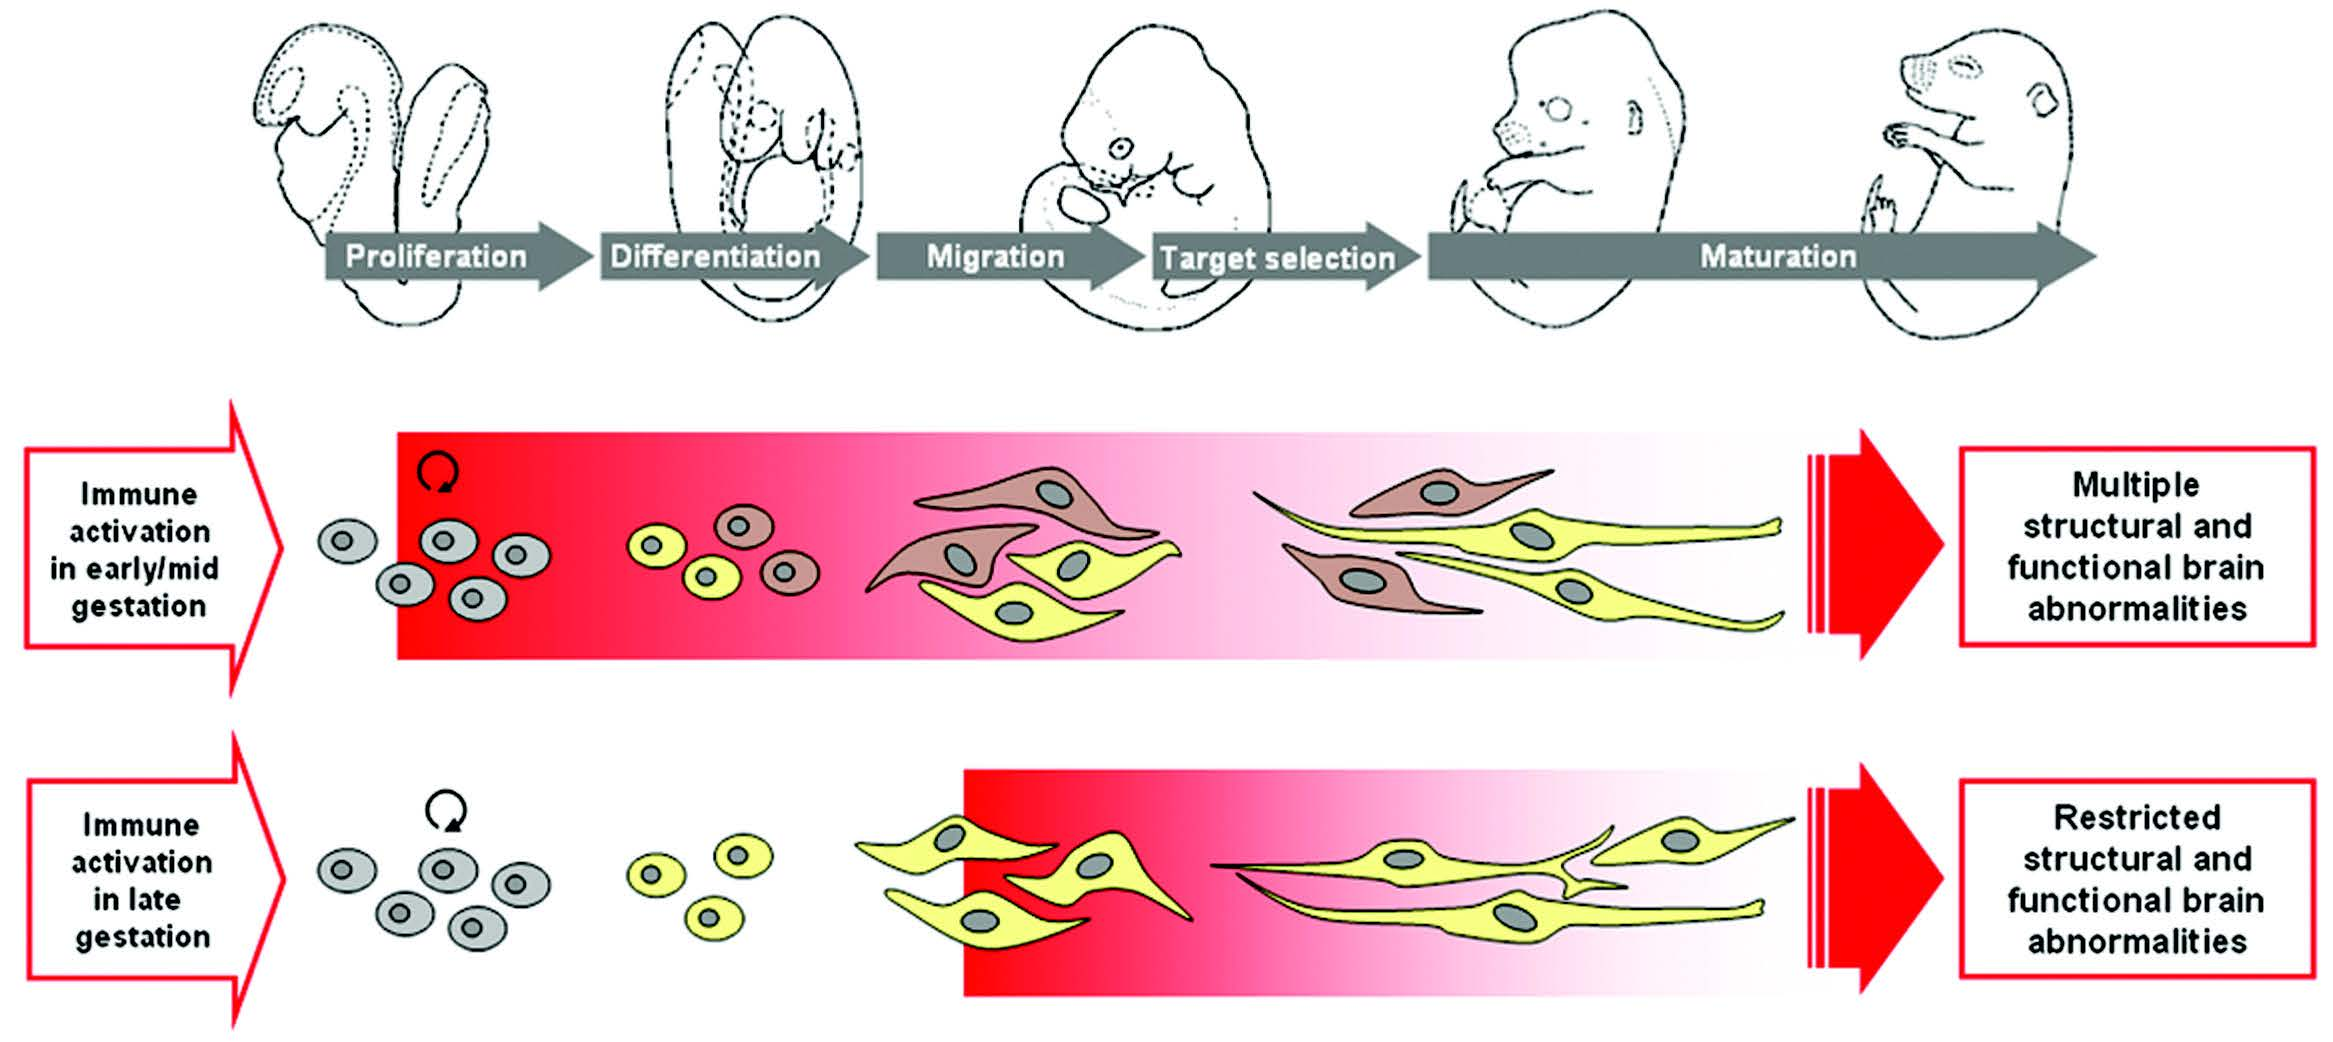
\includegraphics[width=\textwidth]{figure/mia_impact.jpg}
		\caption[Hypothesized model of the impact of prenatal immune challenge on fetal brain development]{Hypothesized model of the impact of prenatal immune challenge on fetal brain development.
			Maternal infection in early/mid pregnancy may affect early neurodevelopmental events in the fetal brain, thereby influencing the differentiation of neural precursor cells (grey) into particular neuronal phenotype (yellow or brown).
			This may predispose the developing fetal nervous system to additional failures leading to multiple structural and functional brain abnormalities in later life.
			Figure used with permission from Journal \citep{Meyer2007a}}
		\label{fig:miaEffect}
	\end{figure}
	
	In a separate study by \citet{Giovanoli2013}, mice were exposed to low dosage of \gls{polyic} during early gestation.
	Offspring born were then left undisturbed or exposed to unpredictable stress during peripubertal development.
	It was observed that offspring exposed to \gls{polyic} has an increased level of dopamine in the nucleus accumbens independent to whether if they were exposed to postnatal stress whereas serotonin (5-HT) were decreased in the medial prefrontal cortex when exposed to postnatal stress regardless of prenatal exposure.
	Only when the offspring were exposed to both \gls{polyic} and postnatal stress will they have an increased dopamine levels in the hippocampus or will sensorimotor gating and psychotomimetic drug sensitivity be affected \citep{Giovanoli2013}.
	\citet{Giovanoli2013} therefore suggest that the prenatal insult serves as a ``disease primer'' that increase offspring's vulnerability to subsequent insults.
	
	Another interesting observation in \citet{Giovanoli2013}'s study was that the combined immune activation and stress led to a 2.5 to 3 fold increase in hippocampal and prefrontal expression of markers characteristic of activated microglia.
	Considering that microglia is responsible for synaptic pruning during brain development \citep{Paolicelli2011}, perturbation of microglia in the fetal brain might also mediate \glng{scz}.
	Indeed, \citet{Onore2014} demonstrated that \gls{mia} has a prolonged effect on macrophages, leading to a shift towards to proinflammatory M1 phenotype.
	Immune dysfunction in the pathophysiology of \glng{scz} has long been speculated \citep{Muller2010a} and evidence shown that there was a strong influence of the pro- and anti-inflammation cytokines on the glutamatergic neurotransmission \citep{Muller2010a}, suggesting the immune system might played an important role in disease etiology of \glng{scz}.
	
	\begin{figure}
		\centering
		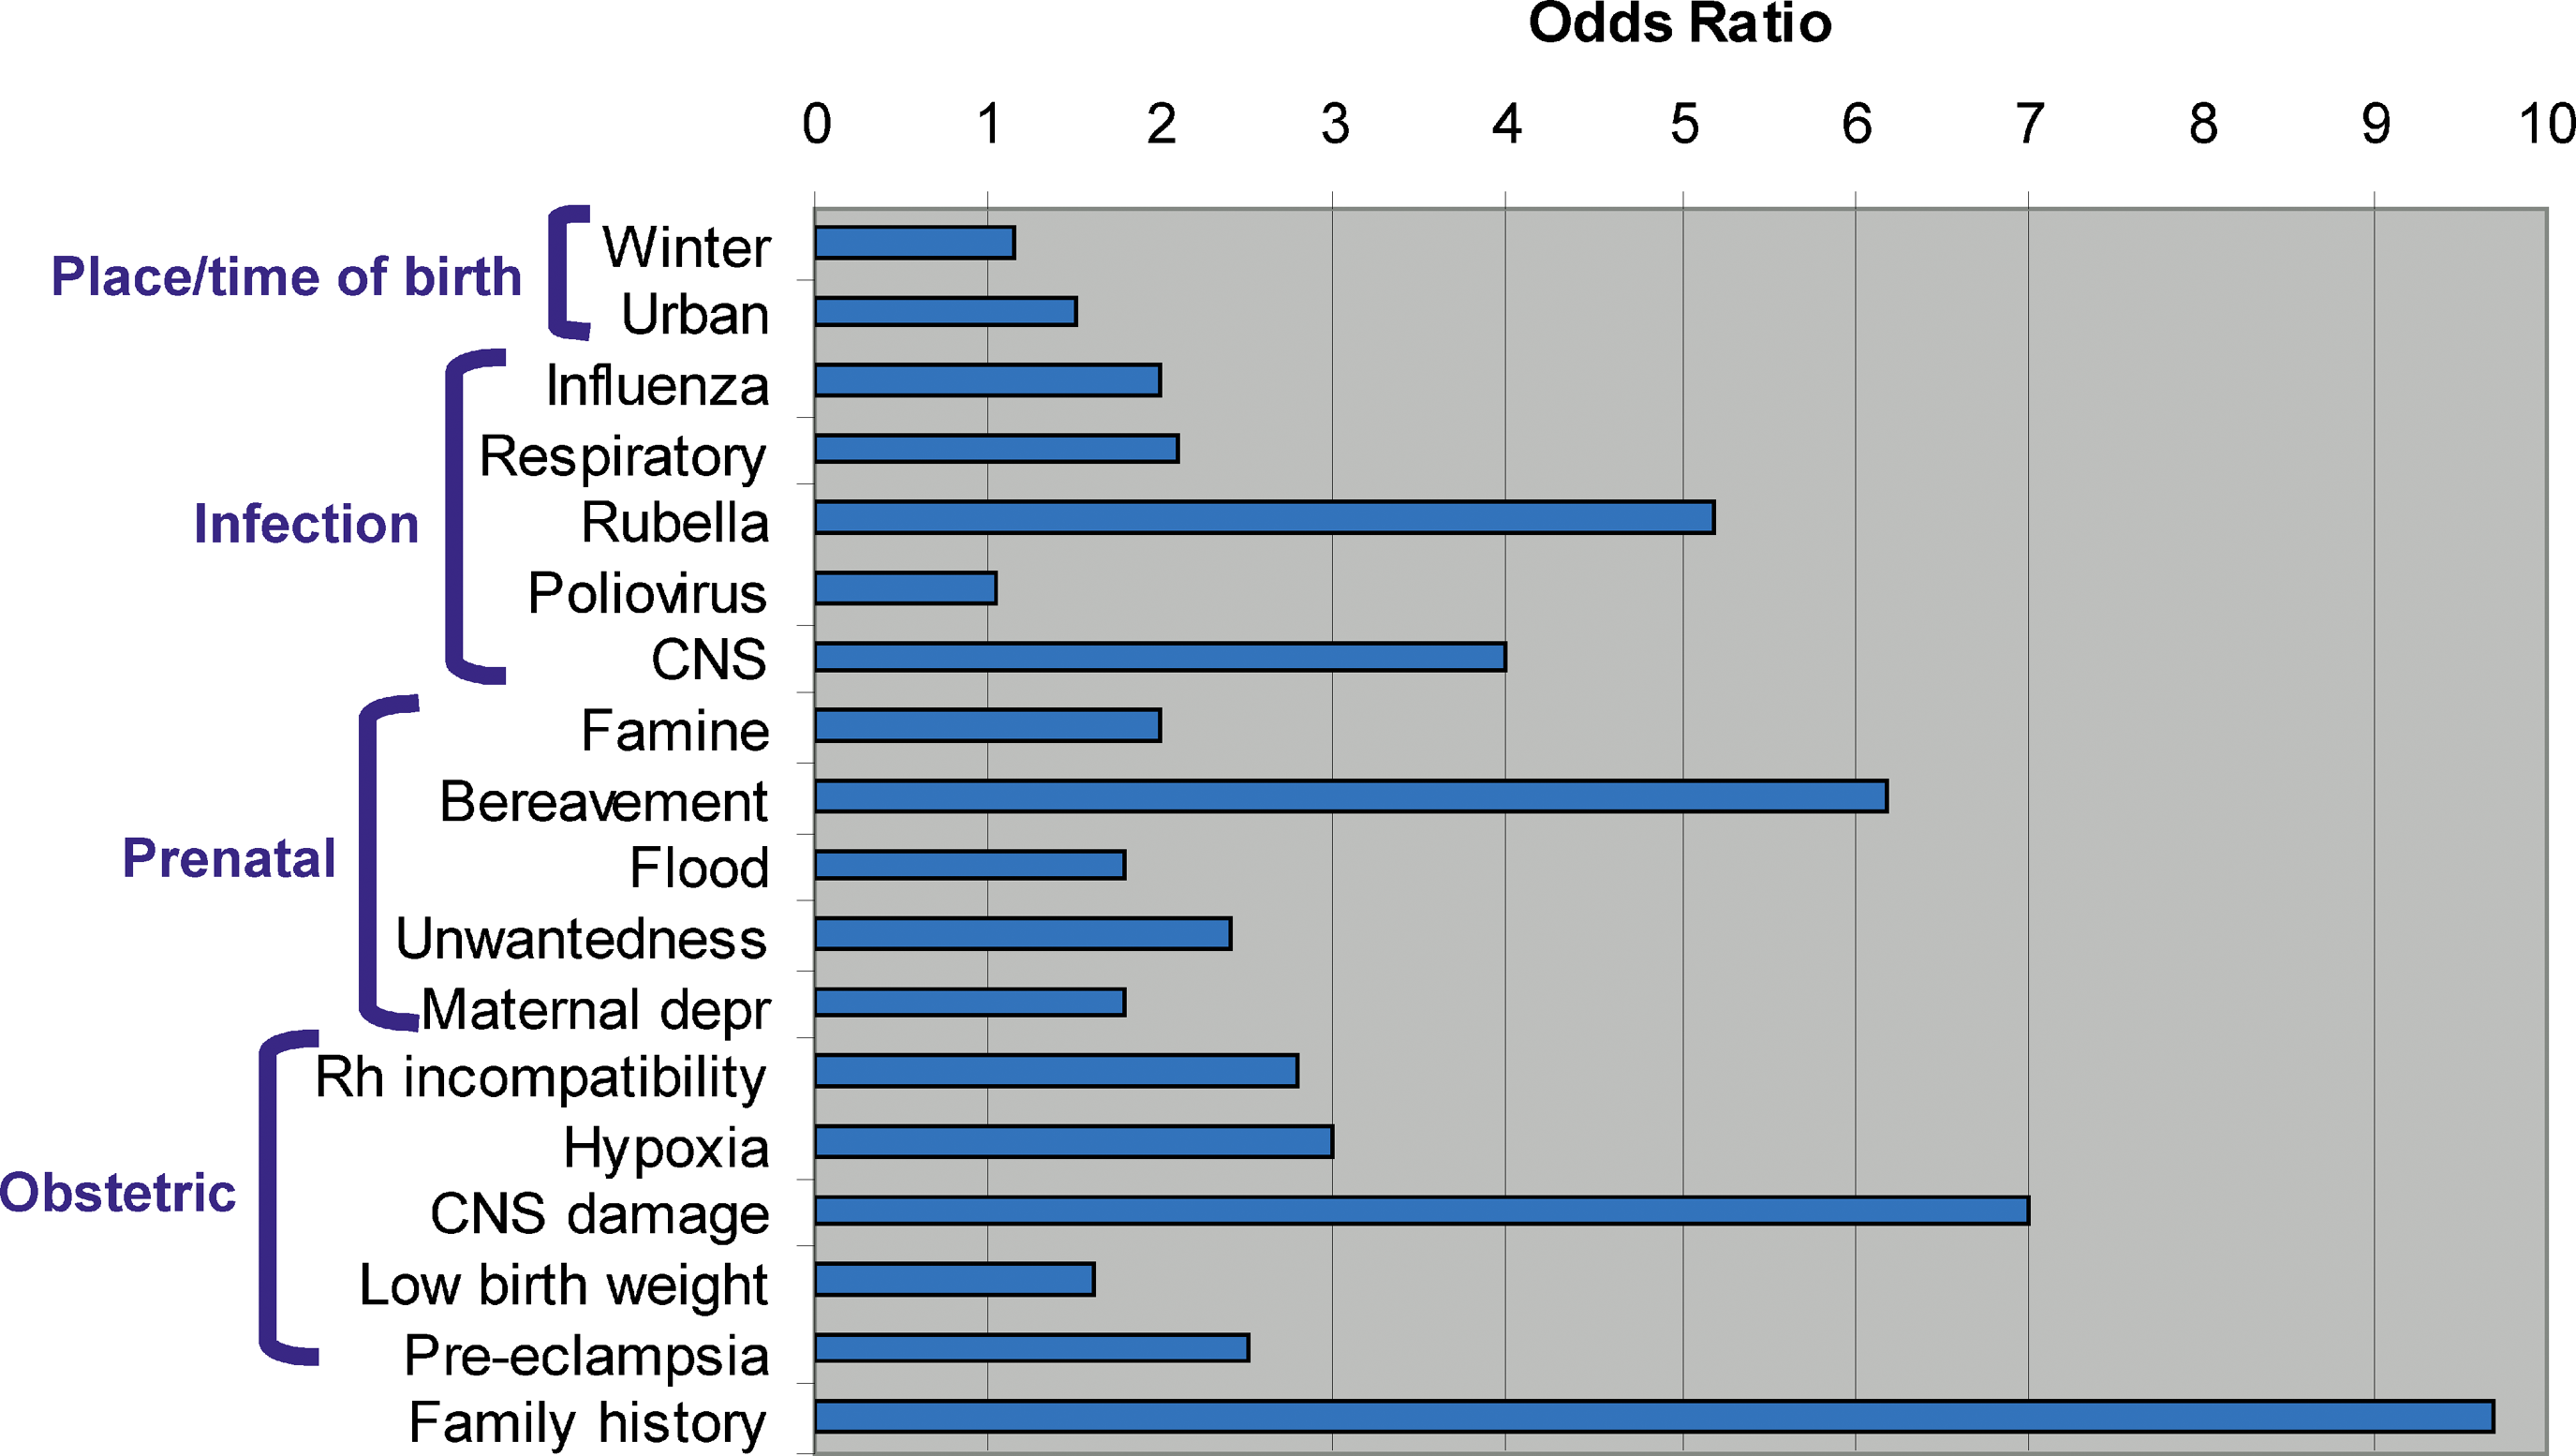
\includegraphics[width=\textwidth]{figure/risk_factors_of_schizophrenia.png}
		\caption[Risk factors of \glng{scz}]{Risk factors of \glng{scz}.
			It was observed that family history of \glng{scz} was the largest risk factors.
			Risk of \glng{scz} can be more than 9 times higher than the general population for individual with a family history of \glng{scz}}
		\label{fig:riskfactors}
	\end{figure}
	
	Together, these results supports the involvement of \gls{mia} in the development of \glng{scz}.
	It was even estimated that one third of all \glng{scz} cases could have been prevented shall all infection were prevented from the entire pregnant population \citep{Brown2010}.
	
	Similarly, tobacco consumption \citep{Kelly1999} and socio economic status were also found to be associated with increased risk of schizophrenia \citep{McGrath2008a}.
	However, by and large, the single largest risk factor was family history of \glng{scz} (\cref{fig:riskfactors}) \citep{Sullivan2005}.
	Studies conducted by Ernst R{\"u}din, Franz J. Kallmann and Hans Luxenburger, all demonstrated that the relatives of \glng{scz} tends to have increased risk of \glng{scz} \citep{Gottesman1982}. 
	The implication of such observation was twofold:
	as family members usually shares larger portion of their genetic effects with each other than that of the population, the genetic effects might be the main mediator of \glng{scz}; 
	on the other hand, culture, socio-economic status and area of birth usually transmit within the family, so one cannot separate the environmental factors from the genetic factors.

	It was important to study the relative contribution of genetic and environmental influence to individual differences in \glng{scz}.
	If \glng{scz} was indeed a genetic disease, one may then focus the resources into study of genetic variations in \glng{scz} patients. 
	To quantify the relative contribution of genetic and environmental influence, one will need to estimate the \emph{heritability} of \glng{scz}.
	